\section{Some background}\label{some-background}

\begin{frame}{Reproducible research}

\begin{quote}
``The term reproducible research refers to the idea that the ultimate
product of academic research is the paper along with the \textbf{full
computational environment used to produce the results in the paper such
as the code, data, etc.} that can be used to reproduce the results and
create new work based on the research''
\end{quote}

\raggedleft 

\href{https://en.wikipedia.org/wiki/Reproducibility\#Reproducible_research}{Wiki}

\begin{figure}
\centering
\includegraphics[width=.5\linewidth]{F1-large.jpg}\\
\footnotesize CREDIT: JOE SUTLIFF/WWW.CDAD.COM/JOE
\end{figure}

\end{frame}

\begin{frame}{Reproducible research (cont.)}

\begin{itemize}
\tightlist
\item
  A major new issue in sciences (overall):

  \begin{itemize}
  \tightlist
  \item
    Accessible Reproducible Research
    (\href{http://science.sciencemag.org/content/327/5964/415}{Mesirov,
    \textbf{Science} 2010})
  \item
    Again, and Again, and Again, \ldots{}
    (\href{http://science.sciencemag.org/content/334/6060/1225}{Jasny et
    al., \textbf{Science} 2011})
  \item
    Challenges in Irreproducible Research
    (\href{http://www.nature.com/news/reproducibility-1.17552}{\textbf{nature}
    topic})
  \end{itemize}
\item
  Not far away from social sciences\ldots{}

  \begin{itemize}
  \tightlist
  \item
    ``Estimating the reproducibility of psychological science''
    (\href{http://science.sciencemag.org/content/349/6251/aac4716}{Nosek
    and a bunch more, \textbf{Science} 2015}{]}): 39\% of replications
    obtained statistically significant results.
  \end{itemize}
\end{itemize}

\end{frame}

\begin{frame}{Concepts}

\begin{itemize}
\item
  Literate programming
\item
\end{itemize}

\end{frame}

\begin{frame}{What can you do?}

\begin{itemize}
\tightlist
\item
  Provide \textbf{raw} data (raw, i.e.~before ``cleaning it''),
\item
  Provide source code (what ever programming environment you are using)
  for reproducing: \emph{cleaned data}, models, tables, figures, etc.
\item
  Hopefully have a neat way of coding your programs: Inline Comments,
  Indentation of control-flow statements (for, while, case, switch,
  ifelse, etc.)
\end{itemize}

\end{frame}

\begin{frame}{What else could you do?}

\begin{itemize}
\tightlist
\item
  Try using version control software (such as git) to make your research
  ``opensource''
\item
  Avoid using proprietary software (hopefully always)
\end{itemize}

\end{frame}

\section{Hands on literate
programming}\label{hands-on-literate-programming}

\begin{frame}{In general}

\begin{itemize}
\tightlist
\item
  LaTeX: Nice typesetting, nice references manager, high quality figures
  (PostScript, PDF), out-of-the-box automation
\item
  Use markdown+pandoc
\end{itemize}

\end{frame}

\begin{frame}{Tools}

\begin{itemize}
\tightlist
\item
  R

  \begin{itemize}
  \tightlist
  \item
    Try using
    \href{https://cran.r-project.org/web/packages/knitr/index.html}{knitr}
    and
    \href{https://cran.r-project.org/web/packages/rmarkdown/index.html}{Rmarkdown}
  \item
    \href{https://cran.r-project.org/web/packages/texreg/index.html}{texreg}
    for fancy regression tables.
  \item
    More resources at CRAN task View
    \href{https://cran.r-project.org/web/views/ReproducibleResearch.html}{Reproducible
    Research}
  \end{itemize}
\item
  Stata

  \begin{itemize}
  \tightlist
  \item
    Neat tables with:
    \href{https://ideas.repec.org/c/boc/bocode/s456416.html}{outreg2}
  \item
    More resources at
    \href{http://www.ats.ucla.edu/stat/stata/latex/}{UCLA's idre}
  \end{itemize}
\end{itemize}

\end{frame}

\begin{frame}[fragile]{Example 1: Reg-like tables in Stata}

\footnotesize

\begin{verbatim}
## 
## . qui sysuse auto
## 
## . outreg2 using mystatatab.tex, replace tex(frag): ///
## >   qui reg price rep78 i.foreign mpg
## mystatatab.tex
## dir : seeout
## 
## . outreg2 using mystatatab.tex, append tex(frag): ///
## >   qui reg price rep78 mpg
## mystatatab.tex
## dir : seeout
## 
## . outreg2 using mystatatab.tex, append tex(frag): ///
## >   qui reg price rep78 i.foreign
## mystatatab.tex
## dir : seeout
\end{verbatim}

\end{frame}

\begin{frame}

\footnotesize

\begin{table}
\centering
\begin{tabular}{lccc} \hline  & (1) & (2) & (3) \\ VARIABLES & price & price & price \\ \hline  &  &  &  \\ rep78 & 432.8 & 667.0* & 76.29 \\  & (394.7) & (342.4) & (449.3) \\ 1.foreign & 1,023 &  & -205.6 \\  & (866.1) &  & (959.5) \\ mpg & -292.4*** & -271.6*** &  \\  & (60.23) & (57.77) &  \\ Constant & 10,586*** & 9,658*** & 5,949*** \\  & (1,556) & (1,347) & (1,423) \\  &  &  &  \\ Observations & 69 & 69 & 69 \\  R-squared & 0.267 & 0.251 & 0.001 \\ \hline \multicolumn{4}{c}{ Standard errors in parentheses} \\ \multicolumn{4}{c}{ *** p$<$0.01, ** p$<$0.05, * p$<$0.1} \\ \end{tabular}
\caption{A regression table with different specifications (stata)}
\end{table}

\end{frame}

\begin{frame}[fragile]{Example 2: Plots in stata}

\footnotesize

\begin{verbatim}
## 
## . qui sysuse auto
## 
## . scatter price mpg, scheme(economist)
## 
## . graph export mystataplot.eps, replace
## (file mystataplot.eps written in EPS format)
\end{verbatim}

\end{frame}

\begin{frame}

\begin{figure}
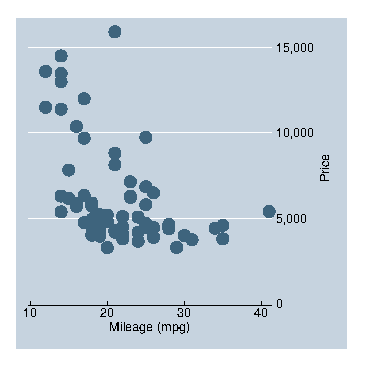
\includegraphics[width=.5\linewidth]{mystataplot.eps}
\caption{A scatter plot from stata using ``The Economist'' scheme}
\end{figure}

\end{frame}

\begin{frame}[fragile]{Example 3: Regression tables in R}

From stata

\footnotesize

\begin{verbatim}
sysuse auto
save auto.dta, replace
\end{verbatim}

\begin{verbatim}
## 
## . sysuse auto
## (1978 Automobile Data)
## 
## . save auto.dta, replace
## file auto.dta saved
\end{verbatim}

\normalsize

Now, in R

\footnotesize

\begin{Shaded}
\begin{Highlighting}[]
\NormalTok{auto <-}\StringTok{ }\NormalTok{foreign::}\KeywordTok{read.dta}\NormalTok{(}\StringTok{"auto.dta"}\NormalTok{)}
\NormalTok{ans1 <-}\StringTok{ }\KeywordTok{lm}\NormalTok{(price~rep78+}\KeywordTok{factor}\NormalTok{(foreign)+mpg, auto)}
\NormalTok{ans2 <-}\StringTok{ }\KeywordTok{lm}\NormalTok{(price~rep78+mpg, auto)}
\NormalTok{ans3 <-}\StringTok{ }\KeywordTok{lm}\NormalTok{(price~rep78+}\KeywordTok{factor}\NormalTok{(foreign), auto)}
\end{Highlighting}
\end{Shaded}

\end{frame}

\begin{frame}

\begin{table}
\scriptsize

\begin{tabular}{l c c c }
\hline
 & Model 1 & Model 2 & Model 3 \\
\hline
(Intercept)            & $10586.48^{***}$ & $9657.75^{***}$ & $5948.78^{***}$ \\
                       & $(1555.74)$      & $(1346.54)$     & $(1422.63)$     \\
rep78                  & $432.80$         & $666.96$        & $76.29$         \\
                       & $(394.71)$       & $(342.36)$      & $(449.27)$      \\
factor(foreign)Foreign & $1023.21$        &                 & $-205.61$       \\
                       & $(866.09)$       &                 & $(959.55)$      \\
mpg                    & $-292.43^{***}$  & $-271.64^{***}$ &                 \\
                       & $(60.23)$        & $(57.77)$       &                 \\
\hline
R$^2$                  & 0.27             & 0.25            & 0.00            \\
Adj. R$^2$             & 0.23             & 0.23            & -0.03           \\
Num. obs.              & 69               & 69              & 69              \\
RMSE                   & 2550.90          & 2558.54         & 2955.15         \\
\hline
\multicolumn{4}{l}{\scriptsize{$^{***}p<0.001$, $^{**}p<0.01$, $^*p<0.05$}}
\end{tabular}
\normalsize
\caption{A regression table with different specifications (R)}
\end{table}

\end{frame}

\begin{frame}[fragile]{Example 4: Plots in R}

\footnotesize

\begin{Shaded}
\begin{Highlighting}[]
\NormalTok{cols <-}\StringTok{ }\NormalTok{auto$rep78}
\NormalTok{cols[}\KeywordTok{is.na}\NormalTok{(cols)] <-}\StringTok{ }\DecValTok{0}
\NormalTok{vran <-}\StringTok{ }\KeywordTok{range}\NormalTok{(cols, }\DataTypeTok{na.rm =} \OtherTok{TRUE}\NormalTok{)}
\NormalTok{cols <-}\StringTok{ }\NormalTok{(cols-vran[}\DecValTok{1}\NormalTok{])/(vran[}\DecValTok{2}\NormalTok{] -}\StringTok{ }\NormalTok{vran[}\DecValTok{1}\NormalTok{])}
\NormalTok{cols <-}\StringTok{ }\KeywordTok{rgb}\NormalTok{(}\KeywordTok{colorRamp}\NormalTok{(blues9)(cols), }\DataTypeTok{maxColorValue =} \DecValTok{255}\NormalTok{)}
\KeywordTok{plot}\NormalTok{(price~mpg, auto, }\DataTypeTok{pch=}\DecValTok{19}\NormalTok{, }\DataTypeTok{col=}\NormalTok{cols)}
\end{Highlighting}
\end{Shaded}

\begin{figure}
\includegraphics[width=.6\linewidth]{reproducible_research_files/figure-beamer/rscatter-1} \caption{A neat plot in R}\label{fig:rscatter}
\end{figure}

\end{frame}
